\documentclass[12pt]{article}

\usepackage[hyphens,spaces,obeyspaces]{url}
\urlstyle{same}
\usepackage{tabularx}
\usepackage{pgfplots}
\pgfplotsset{compat=1.14}
\usepackage{multicol}
\usepackage{caption}
\usepackage{pgfplotstable}
\usepackage{graphicx}
\usepackage{float}
\usepackage[style=numeric,backend=biber]{biblatex}
\addbibresource{ref.bib}
\usepackage[textwidth=528pt]{geometry}
\nocite{*}

	\title{\textbf{Simulating Formula 1 crashes in the start-section including the first turn}}
	\date{\today}
	\author{Kevin Wilbrink (6310621) and Jordi Wippert (6303013)}

\begin{document}
	\maketitle

	\begin{multicols*}{2}
		\textbf{Abstract -- Crashes in Formula 1 are influenced by certain properties of circuits. A computer simulation model, based on the Nagel-Schreckenberg traffic model, is used to study the effects of acceleration, turn speed, distance and braking. The goal is to find unsafe conditions in a small part of a circuit. The results show that crashes are influenced by speed but that there is no significant factor that shows how or when a crash will happen.
}

		\section{Introduction}
		In formula 1 crashes are more a rule than an exception. In the grand prix' [LINK] in 2017 only, half of the races had incidents in the section including the first turn. [LINK] We would like to find out if cars are more likely to crash if the circuit has a certain set of characteristics.

In previous research, various properties of racing are already taken into account, such as regulations and safety measurements on technical level of a car to improve the safety of a driver [LINK]. We hope to find particular causes in the properties of a track, to improve which can be used to reach this same goal.

In order to do this a model for the behaviour of drivers/cars is created and used to simulate races on various tracks under a few circumstances.


		\section{Methods}
		To obtain a view on how the amount of crashes in the first section is influened by various factors, Monte Carlo simulations are being used. Each simulation represents a start of a grand prix, in which every car attempts to pass the first turn. These cars, with an average length of five metres, and a width of two, start at a grid with two sides. Every other car starts left, or right, based on the first (pole) position, with 8 metres in between \cite{car-regulations}, on a so called grid. For our simulation we divided the total width of the circuit in five lanes, to make it possible to take over cars.

There are 20 cars in each race. And in the simulations, every track of the 2017 formula 1 calendar is being tested, 20 in total. The order in which the cars start, is sampled in each simulation out of all achieved qualification results in this season so far (16). By doing this, the possibilty that a driver had a bad day, or penalty can be neglected. When the driver within a team is switched during the season, this will be taken in advance.

To mimic the real world, behaviour of drivers/cars is based on the four steps used in the Nagel-Schreckenberg model;\\

\noindent
(1) acceleration,\\
(2) slowing down,\\
(3) randomization,\\
(4) car motion.\\

As long as the point of where a car should brake isn't reached, the car accelerates (1). The numbers being used to calculate the amount of metres that are added every second, are based on a few cars \cite{som}, and define the range for all cars.

When the 'braking zone' is (nearly) reached, the negative acceleration (2) is being calculated with the current speed of the car and the metres that are needed to brake for this turn on average \cite{som}.

Next to improving the distance driven, there will be attempted to move to an optimal position on the track (4). What's optimal for a car at a certain moment differs. Ideally, if a car is faster than the car in front of him, it will try to take over. Take overs will be done with the "optimal row"\footnote{The opposite side of the turn is considered as being optimal. By driving there, you could maintain the top speed/accelerate as long as possible.} in consideration.

When a car is in front of another car which is considered faster, it will try to defend its position by moving towards the row the car in the back is driving, in order to 'block' it.

Driving into the braking zone also means that an optimal position should be chosen to drive into the turn.

Sometimes when a car is faster, has the plan to defend or to improve its position, other cars are blocking this, or the car needs to go off the track to obtain the result. In this case the current position on track will be maintained.

\subsection{Crashes}
Checks for crash occurences will be executed till the second in which the car has passed the point of the first turn.

A check validates if something happend between the current car, and the car in front of it. By doing this, it's possible to check if the manouvre which just was executed, either accelerating, braking or switching could be performed succesfully.

Crashes can only happen between cars that are in the same row. If a crash is near, an additional switch of rows may be performed to avoid a crash. When no positive options are left, the driver has the option to brake, or crash. A choice out of these two will be made randomly (3). If the distance between the current car and the car in front is less than zero, this will be considered as a crash.


		\section{Results}
		The results are based on simulations which are ran 10,000 times for each track. The total sum of crashes is 121,747.\\

\noindent
\begin{tabularx}{.50\textwidth}{Xlllll}
country    & turn &mtr&brake  &speed &crashes\\
\hline
Australia  & R-L       & 381    &100    &150   &7837\\
Austria    & R-L       & 318    &200    &122   &673\\
Azerbaijan & L-R       & 206    &50     &116   &7926\\
Bahrain    & R-L       & 476.4  &100    &70    &7792\\
Belgium    & R-L       & 251    &150    &77    &2887\\
Brazil     & L-R       & 334    &50     &109   &5129\\
Canada     & R-L       & 258    &125    &154   &6334\\
China      & R-L       & 324.7  &50     &170   &7664\\
GBR        & R-L       & 270    &-      &281   &991\\
Hungary    & R-L       & 576    &100    &85    &7550\\
Italy      & R-L       & 615    &125    &80    &7393\\
Japan      & R-L       & 373    &10     &152   &1262\\
Malaysia   & R-L       & 620    &100    &74    &8849\\
Monaco     & R-R       & 111    &75     &103   &7477\\
Russia     & R-R       & 205.2  &-      &300   &2103\\
Spain      & R-L       & 690.5  &100    &130   &7211\\
Mexico     & R-L       & 890    &200    &107   &6279\\
Singapore  & L-L       & 274    &50     &126   &8724\\
UAE        & L-R       & 305    &50     &150   &9449\\
USA        & L-R       & 364    &100    &86    &8217\\
\end{tabularx}
\captionof{table}{Overview of grand prix, with circuit data. Column 'turn' defines sides, left or right, for both the first turn and the pole position.}\label{table:results}\\

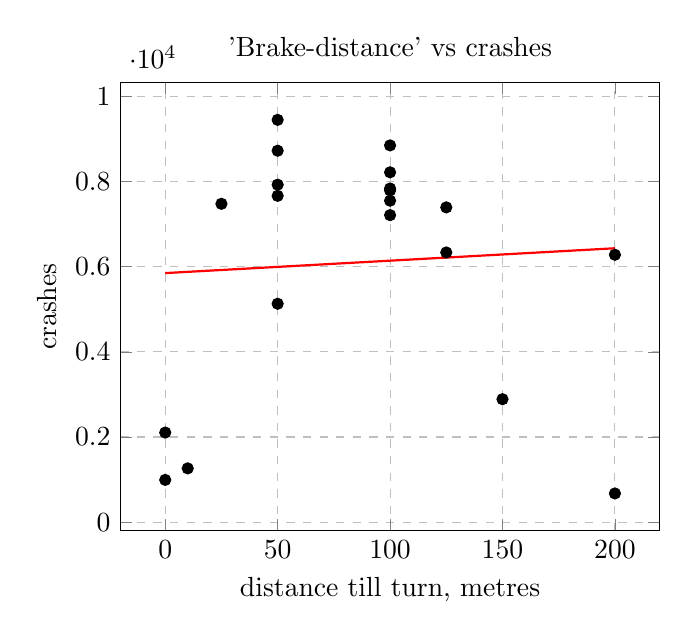
\begin{tikzpicture}
\begin{axis}[
  title={'Brake-distance' vs crashes},
  xlabel={distance till turn, metres},
  ylabel={crashes},
  ymajorgrids=true,
  xmajorgrids=true,
  grid style=dashed,
]
\addplot[ only marks ]
  coordinates {(0,991)(0,2103)(10,1262)(25,7477)(50,7926)(50,5129)(50,7664)(50,8724)(50,9449)(100,7837)(100,7792)(100,7550)(100,8849)(100,7211)(100,8217)(125,6334)(125,7393)(150,2887)(200,673)(200,6279)};
  \addplot [thick, red] table[y={create col/linear regression}]{
    0 991
    0 2103
    10 1262
    25 7477
    50 7926
    50 5129
    50 7664
    50 8724
    50 9449
    100 7837
    100 7792
    100 7550
    100 8849
    100 7211
    100 8217
    125 6334
    125 7393
    150 2887
    200 673
   };
\end{axis}
\end{tikzpicture}
\captionof{figure}{Distance in metres before a turn that is used on average to brake before turn one to achieve the right speed, plotted against the amount of crashes.}\label{fig:results1}

\medskip
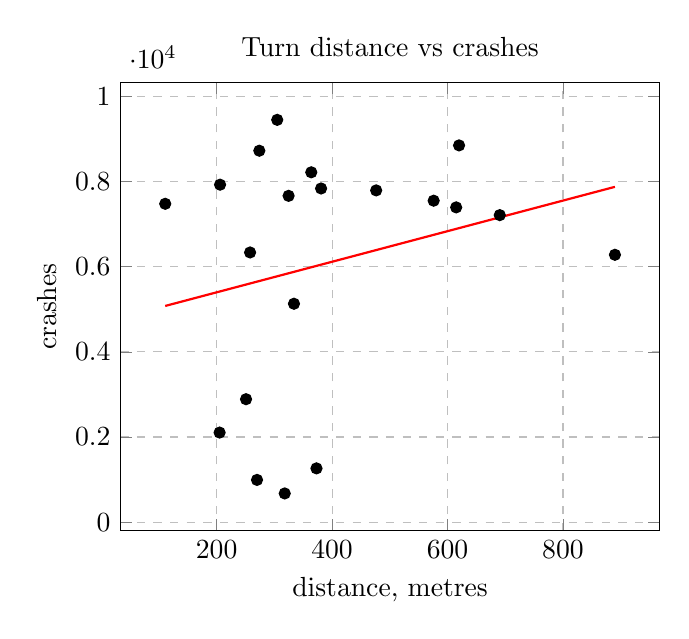
\begin{tikzpicture}
\begin{axis}[
  title={Turn distance vs crashes},
  xlabel={distance, metres},
  ylabel={crashes},
  ymajorgrids=true,
  xmajorgrids=true,
  grid style=dashed,
]
\addplot[ only marks ]
  coordinates {(111,7477)(205.2,2103)(206,7926)(251,2887)(258,6334)(270,991)(274,8724)(305,9449)(318,673)(324.7,7664)(334,5129)(364,8217)(373,1262)(381,7837)(476.4,7792)(576,7550)(615,7393)(620,8849)(690.5,7211)(890,6279)};
  \addplot [thick, red] table[y={create col/linear regression}]{
    111 7477
    205.2 2103
    206 7926
    251 2887
    258 6334
    270 991
    274 8724
    305 9449
    318 673
    324.7 7664
    334 5129
    364 8217
    373 1262
    381 7837
    476.4 7792
    576 7550
    615 7393
    620 8849
    690.5 7211
    890 6279
  };
\end{axis}
\end{tikzpicture}
\captionof{figure}{Distance in metres calculated from start-line till first turn, plotted against the amount of crashes.}\label{fig:results2}

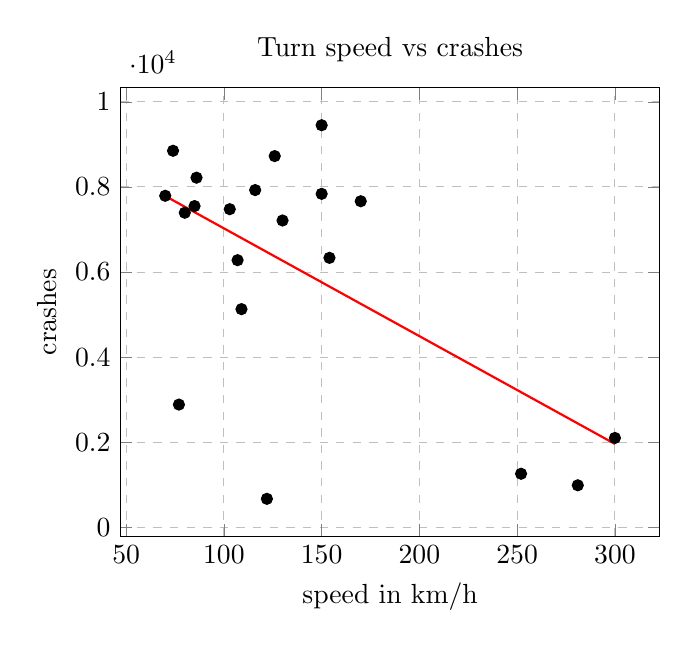
\begin{tikzpicture}
\begin{axis}[
  title={Turn speed vs crashes},
  xlabel={speed in km/h},
  ylabel={crashes},
  ymajorgrids=true,
  xmajorgrids=true,
  grid style=dashed,
]
\addplot[ only marks ]
  coordinates {(70,7792)(74,8849)(77,2887)(80,7393)(85,7550)(86,8217)(103,7477)(107,6279)(109,5129)(116,7926)(122,673)(126,8724)(130,7211)(150,7837)(150,9449)(154,6334)(170,7664)(252,1262)(281,991)(300,2103)};
  \addplot [thick, red] table[y={create col/linear regression}]{
    70 7792
    74 8849
    77 2887
    80 7393
    85 7550
    86 8217
    103 7477
    107 6279
    109 5129
    116 7926
    122 673
    126 8724
    130 7211
    150 9449
    150 7837
    154 6334
    170 7664
    252 1262
    281 991
    300 2103
  };
\end{axis}
\end{tikzpicture}
\captionof{figure}{Maximum speed that should be driven in turn to achieve best result, plotted against crashes.}\label{fig:results3}


    \section{Discussion \& conclusion}
		All the circuits of 2017 are listed in table \ref{table:results}, with the corresponding data. The last column shows the amount of crashes, computed by the simulations. The number of crashes seems divided equally over the circuits. This is in line with the real-world amount of crashes this season so far.

Figure \ref{fig:results1} shows an almost horizontal line in the distance that is being used to brake before the turn. This indicates that the amount of metres that is shown on the track by brake-pads/distance indicators, seems right and doesn't affect the amount of crashes.

According to figure \ref{fig:results2}, we see that the number of crashes increase when the distance of a turn calculated from start rises. There are numerous causes for this, high speed could be one. Putting it in perspective, you could also say that there's more metres to crash, so it's logical that the number gets higher.

The higher the speed that could be maintained in a turn, the lower the number of crashes, Figure \ref{fig:results3} describes. This can be explained by the descreased brake time for a car, which doesn't cause head-tail collisions anymore.

The combined results show that the amount of crashes varies among speeds and (brake) distances, but no hard correlation can be found. E.g. when a turn is far away from the start, but needs a low speed, with long braking distance, it could have the same outcome as when this turn is right after start. This tells us that we find no hard (safety) reasons why the FIA prefers to have a turn at least 250 metres.

By improving the model, with futher research, and adding extra conditions like driver response times, width's of the corners and weather circumstances, it might be possible to find correlations. Also, a better model for acceleration can be used, where it's now linear. Next to that, there are regulations for defending a position, which state that you can't switch sides unlimited. Also it might be a good idea to improve the study on for example all crashes on one certain circuit, and extend that, instead of trying to compare all circuits at once.

Our research set a step beyond the well-known traffic model and tries to simulate under harder conditions. This attempt wasn't perfect but indicates how the well known Nagel-Schreckenberg model can be used in more difficult situations. Also can be concluded that it's hard to tell which exact combination of properties should be used to have a first turn with few crashes.


		\section*{Appendix}
		Appendix

		\section*{Acknowledgements}
		Thank people, teacher e.g.

We would like to thank (title) Barkemar for his lectures about how to research a topic based on MC. We would also like to thank (title) Veldhorst for the 'hoorcollege' and answering all of our questions. (something like this?)

		References
	\end{multicols*}
\end{document}
